
\documentclass[final]{beamer}



\usepackage[scale=0.8,size=a1]{beamerposter} % Use the beamerposter package for laying out the poster

\usetheme{confposter} % Use the confposter theme supplied with this template
\usepackage{multicol}
\setbeamercolor{block title}{fg=dblue,bg=white} % Colors of the block titles
\setbeamercolor{block body}{fg=black,bg=white} % Colors of the body of blocks
\setbeamercolor{block alerted title}{fg=white,bg=dblue!70} % Colors of the highlighted block titles
\setbeamercolor{block alerted body}{fg=black,bg=dblue!10} % Colors of the body of highlighted blocks
% Many more colors are available for use in beamerthemeconfposter.sty

%-----------------------------------------------------------
% Define the column widths and overall poster size
% To set effective sepwid, onecolwid and twocolwid values, first choose how many columns you want and how much separation you want between columns
% In this template, the separation width chosen is 0.024 of the paper width and a 4-column layout
% onecolwid should therefore be (1-(# of columns+1)*sepwid)/# of columns e.g. (1-(4+1)*0.024)/4 = 0.22
% Set twocolwid to be (2*onecolwid)+sepwid = 0.464
% Set threecolwid to be (3*onecolwid)+2*sepwid = 0.708

\newlength{\sepwid}
\newlength{\onecolwid}
\newlength{\twocolwid}
\newlength{\threecolwid}
\setlength{\paperwidth}{33.1in} % A0 width: 46.8in
\setlength{\paperheight}{23.4in} % A0 height: 33.1in
\setlength{\sepwid}{0.0\paperwidth} % Separation width (white space) between columns
\setlength{\onecolwid}{0.22\paperwidth} % Width of one column
\setlength{\twocolwid}{0.464\paperwidth} % Width of two columns
\setlength{\threecolwid}{0.708\paperwidth} % Width of three columns
\setlength{\topmargin}{-0.5in} % Reduce the top margin size
%-----------------------------------------------------------

\usepackage{graphicx}  % Required for including images

\usepackage{booktabs} % Top and bottom rules for tables

%----------------------------------------------------------------------------------------
%	TITLE SECTION 
%----------------------------------------------------------------------------------------

\title{Heuristique model to study variance in cultural transmission of potery making} % Poster title

\author{Maria Coto-Sarmiento, Simon Carrignon and Xavier Rubio-Campillo} % Author(s)

\institute{Barcelona Supercomputing Center - University of Barcelona} % Institution(s)

%----------------------------------------------------------------------------------------

\begin{document}

\addtobeamertemplate{block end}{}{\vspace*{2ex}} % White space under blocks
\addtobeamertemplate{block alerted end}{}{\vspace*{2ex}} % White space under highlighted (alert) blocks

\setlength{\belowcaptionskip}{2ex} % White space under figures
\setlength\belowdisplayshortskip{2ex} % White space under equations

\begin{frame}[t] % The whole poster is enclosed in one beamer frame

\begin{columns}[t] % The whole poster consists of three major columns, the second of which is split into two columns twice - the [t] option aligns each column's content to the top

\begin{column}{\sepwid}\end{column} % Empty spacer column

\begin{column}{\onecolwid} % The first column

%----------------------------------------------------------------------------------------
%	OBJECTIVES
%----------------------------------------------------------------------------------------

\begin{block}{Introduction}

Cultural evolution theories \cite{mesoudi} provide a set of methods that can be used to account these dynamic of changes, focused on the production of olive oil amphorae during the Roman Empire. 
To achieve this goal, multivariate methods were used to evaluate the differences on the pattern production among pottery workshops \cite{agui}. \\
Specifically we want to identify the origin of these changes and if these changes were produced by cultural reasons depending on the spatial distance and other cultural constraints. As hypothesis, we propose that spatial distribution of pottery workshops is the main influence of the making techniques processes \cite{schillinger}. Four pottery workshops, showed in the map \textbf{(fig.1)} were studied from different spaces in \emph{Baetica}. 
\end{block}

\begin{figure}
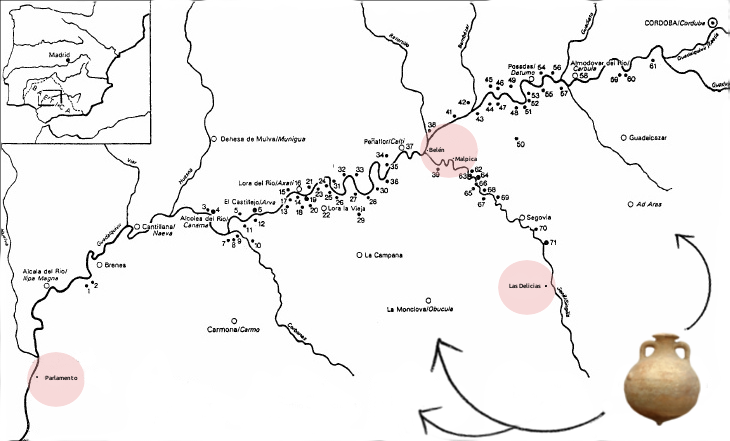
\includegraphics[width=0.6\linewidth]{images/fig1.png}
\caption{Distribution map of the four amphorae workshops. The names  are Las Delicias (\'Ecija, Seville), Bel\'en and Malpica (Palma del R\'io, C\'ordoba) and Parlamento (Seville)}
\end{figure}


\begin{block}{Methods}

{\textbf{Measurements}} \\

To explore the dynamic of changes we analysed a set of measures among different kinds of amphorae shapes from different workshops. We analysed 413 samples of amphorae from 4 different workshops. These workshops were selected from different spaces of \emph{Baetica} area in order to know if there were differences depending on the space. A database was created using a selection of 80 to 90 samples from each pottery workshops. In each sample of amphora we measured eight measurements among different part of the rim being focused on the rim of the amphora. 


\end{block}
\end{column} % End of the first column

%BEGIN THE SECOND COLUMN-------------------------------------------------


\begin{column}{\sepwid}\end{column} % Empty spacer column

\begin{column}{\twocolwid} % Begin a column which is two columns wide (column 2)


\begin{block}{}

\begin{columns}

\begin{column}{0.48\textwidth}
\justify
In each sample of amphora we measured eight measurements among different part of the rim being focused on the rim of the amphora.
\\
{\textbf{Multivariate method}} \\
\\
\justify
Multivariable methods were used to explore these metrical observations \cite{li}
\end{column}

\begin{column}{0.48\textwidth}
\justify
with the eight measurements as variables.\\ 
Principal Component Analysis allowed us to simplify the dataset to see which variable were more relevant. 
Our results suggested that first and second principal component were more relevant than the rest. 
\end{column}

\end{columns}

\end{block}
 % End of column 2.1


%----------------------------------------------------------------------------------------
%	IMPORTANT RESULT
%----------------------------------------------------------------------------------------

\begin{block}{Results}
\begin{columns}
\begin{column}{0.48\textwidth}

\justify
Several multivariate methods were used such as Principal Component Analysis and Discriminant Analysis to classify. These methods allowed us to know the differences on the pattern production among workshops.In our case, the first two principal components were taken to see the significal differences among workshops depending on the space. The \textbf{figure 2} shows the workshops with a minor space such Bel\'en and Malpica share more pottery traits than the rest: Parlamento and Las Delicias.

\begin{figure}
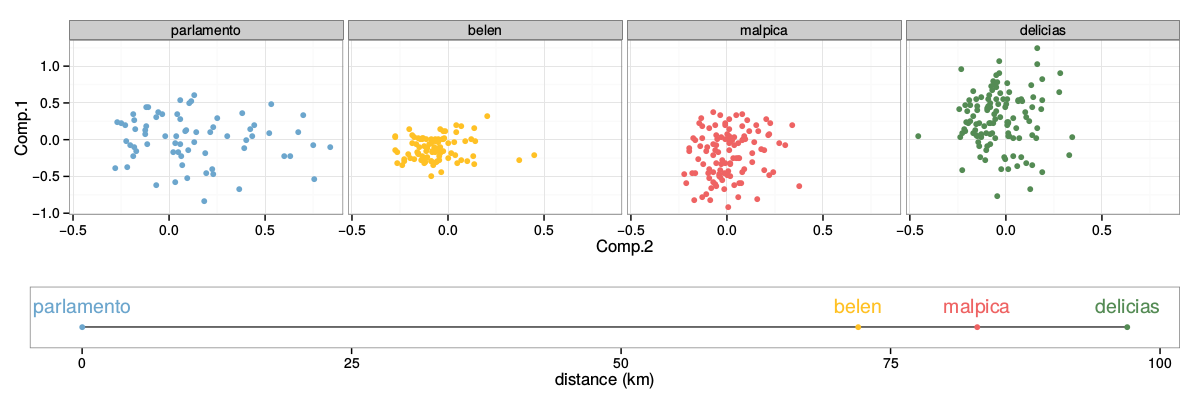
\includegraphics[width=0.7\linewidth]{images/fig2.png}
\caption{Plot with the results of the first two principal components given by the PCA}
\end{figure}

Once defined the components, we used Discriminant Analysis to find a combination among them to define the groups as well as possible. These results were translated to a confusion matrix which basically means what results were predicted as true or false on the discriminant analysis. 

\end{column}

\begin{column}{0.48\textwidth}

\justify

 Thus the system had troubles to distinguishing between Bel\'en and Malpica which had a higher number of confusion or number instead of Parlamento with a minor confusion than the rest. 

 
\begin{figure}
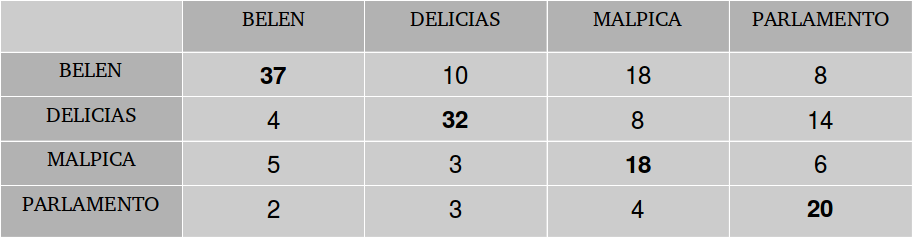
\includegraphics[width=0.6\linewidth]{images/fig3.png}
\caption{Matrix of confusion. Accuracy: 0.5573. P-Value: 0.0006991.}
\end{figure}

\justify
As shown in the \textbf{figure 3} of confusion, all correct guesses were located in the diagonal of the table.\\
A peer to peer comparison was developed among different workshops. We calculated the geographical distance between each site and the distance among pottery measures, calculated using the previous results. The \textbf{figure 4}  shows that the pottery distance is correlated with the spatial distance of workshops.  

\begin{figure}
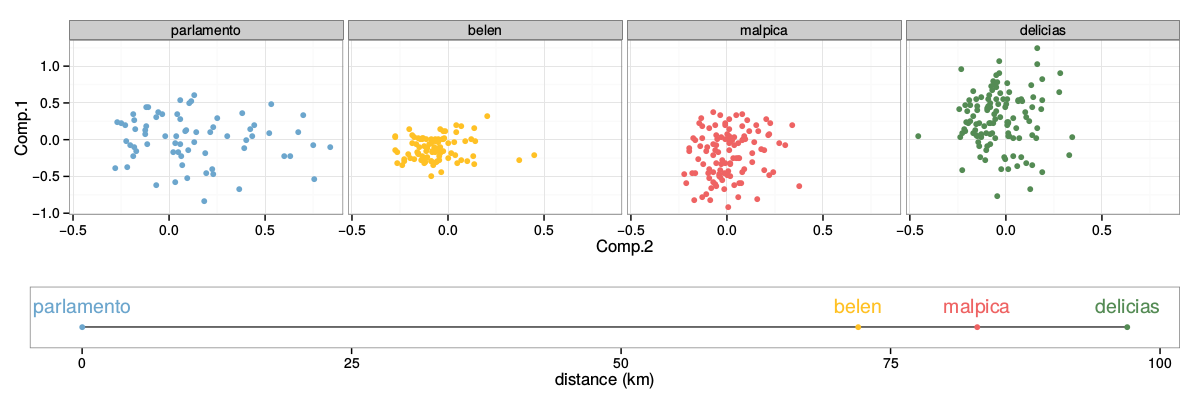
\includegraphics[width=0.7\linewidth]{images/fig2.png}
\caption{Distance metrics calculated among different workshops.}
\end{figure}

 
\end{column}
\end{columns}

\end{block} 

%----------------------------------------------------------------------------------------

\begin{columns}[t,totalwidth=\twocolwid] % Split up the two columns wide column again

\begin{column}{\onecolwid} % The first column within column 2 (column 2.1)


\end{column} % End of column 2.1

\begin{column}{\onecolwid} % The second column within column 2 (column 2.2)


\end{column} % End of column 2.2

\end{columns} % End of the split of column 2

\end{column} % End of the second column




%BEGIN THIRD COLUMN----------------------------------------------------

\begin{column}{\sepwid}\end{column} % Empty spacer column

\begin{column}{\onecolwid} % The third column

\begin{block}{Concluding Remarks}

Differences among pottery workshops were identified using PCA and Discriminant Analysis. As results, Amphorae made in nearby workshops with a minor spacial distance, such as Malpica and Bel\'en, share more traits than amphorae made in pottery workshops farther as Parlamento. It could suggest that the pottery techniques were learned from master to disciple instead of workers with the same level . 

\end{block}

\begin{block}{References}
\small

\bibitem[1]{mesoudi}\textsc{Mesoudi, A. (2015)}
\textit{Cultural Evolution: A review of Theory, Finding and Controversies}, Evolutionary biology.

\bibitem[2]{agui}\textsc{Aguilera, A. (1998)}
\textit{An\'alisis multivariable: una nueva v\'ia para la caracterizaci\'on cer\'amica}, Pyranae, 29.

\bibitem[3]{schillinger}\textsc{Schillinger, K. et al. (2006)}
\textit{Differences in Manufacturing Traditions and Assemblage-Level Patterns: the Origins of Cultural Differences in Archaeological Data}, Journal of Archaeological Method Theory.

\bibitem[4]{li}\textsc{Li, A. (2014)}
\textit{Crossbows and imperial craft organisation: the bronze triggers of China's Terracotta Army}, Antiquity, 88.339.


\end{block}

%----------------------------------------------------------------------------------------
%	ACKNOWLEDGEMENTS
%----------------------------------------------------------------------------------------

\setbeamercolor{block title}{fg=dblue,bg=white} % Change the block title color

\begin{block}{Acknowledgements}

\small{\rmfamily{The Funding for this work was provided by the ERC Advanced Grant EPNet (340828). We thank Museum of \'Ecija and Museum of Palma del R\'io for their assistance. We also thank to dr. Enrique Garc\'ia Vargas (University of Seville) for his helpful suggestions.}} \\

\end{block}

%----------------------------------------------------------------------------------------
%	CONTACT INFORMATION
%----------------------------------------------------------------------------------------

\setbeamercolor{block alerted title}{fg=white,bg=dblue!70} % Change the alert block title colors
\setbeamercolor{block alerted body}{fg=black,bg=white} % Change the alert block body colors

\begin{alertblock}{Contact Information}

\begin{figure}

\includegraphics[width=0.1\linewidth]{images/qrplanet.png}
\end{figure}
\begin{center}
 \href{mailto:maria.coto@bsc.es}{maria.coto@bsc.es}
\end{center}


\end{alertblock}

\begin{center}
\begin{tabular}{ccc}

\includegraphics[width=0.4\linewidth]{images/epnet.png} & \hfill & 
\includegraphics[width=0.4\linewidth]{images/erc.png}
\end{tabular}
\end{center}

%----------------------------------------------------------------------------------------

\end{column} % End of the third column

\end{columns} % End of all the columns in the poster

\end{frame} % End of the enclosing frame

\end{document}
